\chapter{Computational Geometry}
%\chapter{From Contiguous Art Galleries to Convex Hull Peeling}
\label{chap:geom_algos}

In Chapter~\ref{chap:EM_and_persistent_data_structures}, we saw how geometric techniques can be instrumental in designing efficient persistent data structures. 
This chapter now shifts focus to present our contributions to the field of pure computational geometry. 
First, Section~\ref{sec:Area-Weighted Convex Hull Peeling} details an efficient heuristic algorithm for outlier detection in two-dimensional point sets. 
This work, motivated by challenges in computational biology, is based on the principle of area-weighted convex hull peeling. 
Second, Section~\ref{sec:The Contiguous Art Gallery Problem} resolves a recently posed open problem by showing that the contiguous art gallery problem can be solved in polynomial time. 
Our solution is a simple greedy algorithm that is iterated until an optimal set of guards is found. 
The proof of correctness, however, relies on a complex analysis of the geometric and combinatorial properties of the greedy strategy. 
Together, these works showcase two distinct facets of the field. The first leans toward practical application, while the second is entirely theoretical.

\section{Area-Weighted Convex Hull Peeling}
\label{sec:Area-Weighted Convex Hull Peeling}
In this section, we present the contributions of Manuscript~\ref{chap:peeling}. 
The main result is an efficient real-RAM algorithm for area-weighted convex hull peeling in the plane. 
Given a set $P$ of $n$ points, the algorithm iteratively deletes the point with maximum \emph{sensitivity}, defined for a point $p \in P$ as $\sens{p} = \mathrm{area}(\mathrm{CH}(P)) - \mathrm{area}(\mathrm{CH}(P \setminus {p}))$, that is, the decrease in the area of the convex hull when $p$ is removed. Figure~\ref{fig:peeling_datastructures_sensitivity} illustrates the sensitivity of a point.
The removed point is always on the convex hull, and its removal is known as a \emph{peel}~\cite{peeling_layers1, shamos1978thesis}. 
At each step, the algorithm peels the point with maximum sensitivity. 
The algorithm proceeds as follows:

\begin{samepage}
\begin{enumerate}
    \item Initialize the set $P$ to contain all $n$ input points.
    \item Repeat the following $n$ times:
    \begin{itemize}
        \item Identify the point $u = \operatorname*{argmax}_{p \in P} \sens{p}$.
        \item Update $P \leftarrow P \setminus \{u\}$.
    \end{itemize}
\end{enumerate}
\end{samepage}


Depending on the application, the algorithm may be terminated after $k$ iterations, and may output the order in which points are removed from $P$ and the area of the convex hull at each step.

The algorithm is based on the principle that outliers can be detected as points that cause a large decrease in the area of the convex hull when peeled. 
For any parameter $0 < k < n$, our algorithm identifies $k$ outliers by the first $k$ peels, and runs in $\Oh{n \log n}$ time. 
Using the area of the convex hull for outlier detection has been previously explored, primarily from the perspective of identifying the $k$ points whose collective removal causes the largest decrease in area. 
We refer to such a removal as a \emph{$k$-peel}. 
In contrast, our algorithm repeatedly performs $k$ individual $1$-peels, and can be viewed as an efficient \emph{heuristic} for the \emph{exact} computation of a single $k$-peel. 
Note that the exact $k$-peel always produces a convex hull whose area is less than or equal to that obtained by performing $k$ sequential $1$-peels. 
However, the phenomenon of \emph{outlier masking}~\cite{4781136, murphy1951tests, AcunaRodriguez2004}, in which nearby outliers obscure one another, can cause the difference in resulting area between the two approaches to become arbitrarily large. 
The computational complexity of existing exact algorithms and our heuristic is summarized in Table~\ref{tab:k_peeling_table}. 

\begingroup
\begin{table}[ht]
  \centering
  \setlength{\tabcolsep}{0.7em}
  \renewcommand{\arraystretch}{1.5}
  \begin{tabular}{lcc} 
    & Time & Space \\
    \hline
    \textbf{Exact algorithms} \\
    Eppstein~\cite{1992_Eppstein_k3n2, 1992_eppstein_kn3}
    & $\Oh{n^2 \log n + (n - k)^3}$
    & $\Oh{n \log n + (n - k)^3}$ \\ 
    Atanassov et al.%, Bose, Couture,\\ Maheshwari, Morin,\\ Paquette, Smid, Wuhrer.
    ~\cite{2009_Atanassov_exact_small_k}
    & $\Oh{n \log n + \binom{4k}{2k}(3k)^k n}$
    & --- \\[1ex]
    \textbf{Heuristic algorithms} \\
    \emph{Sridhar and Svenning~\cite{20c9233b1df84e03a3ed7cdcdc15ee42}}
    & $\Oh{n \log n}$
    & $\Oh{n}$ \\
    \hline
  \end{tabular}
    \caption{
    Time and space bounds for exact and heuristic $k$-peeling algorithms. 
    The space usage of Atanassov et al.\ was not stated.
    }
  \label{tab:k_peeling_table}
\end{table}
\endgroup

We emphasize that for most values of $n$ and $k$, our algorithm is the first practically viable algorithm. 
The exact methods are combinatorial in nature, whereas our algorithm is a greedy algorithm using dynamic convex hull data structures. 
To prove its efficiency we employ a novel amortized analysis. 
All algorithms generalize to other natural measures such as the perimeter of the convex hull. 

\subsection{Sensitivity}
The sensitivity of a hull point $u$ is determined by its own position, its neighbors on $L_1$, and its \emph{active points}. 
A point $v$ is said to be active for $u$ if it contributes to $\sens{u}$, which means that peeling $u$ would cause $v$ to appear on the convex hull. 
We denote the set of such points by $A(u)$, which consists precisely of the points on the second convex layer $L_2$~\cite{1057060} that would advance to the first layer $L_1$ upon removal of $u$. 
Furthermore, only the points on $L_1$ have positive sensitivity, and the sensitivity of all points depends solely on the set $L_1 \cup L_2$. 
It is therefore surprising that an $\Oh{n \log n}$ time algorithm exists. 
This is because a single peel can cause $\OhMega{n}$ combinatorial changes to $A(u)$ for a single point, and the number of points whose sensitivity changes can also be $\OhMega{n}$. 
Figure~\ref{fig:compute_new_sensitivity} illustrates this behavior and shows how the sensitivity of a point can be updated in time proportional to the number of changes to its active points. 
The core technical part of our analysis is Theorem~\ref{thm:bounding_active_points_amortized}, which bounds the total number of combinatorial changes to active points over the entire course of the peeling process. 
\begin{theorem}~\label{thm:bounding_active_points_amortized}(Manuscript~\ref{chap:peeling}) 
    For any 2D convex hull peeling process on $n$ points, the total number of times any point becomes active for another point is at most~$3n$. 
\end{theorem}

\begin{figure}[ht]
        \centering
        \includegraphics[scale=0.14]{My_Chapters/geom_figs/Case 2 Alt.png}
        \caption{
        Before peeling $v$, the sensitivity $\sens{u}$ is determined by the area of the polygon $\poly{t \circ u \circ v \circ u_e \circ A(u)}$, where $\circ$ denotes the concatenation of vertices. After $v$ is peeled, $\sens{u}$ can be updated in $\Oh{\size{\Delta A}}$ time by subtracting the area of the red triangle $\Tri{u}{v}{q}$ and adding the area of the green polygon $\poly{u_e \circ q \circ v' \circ \Delta A}$. 
        All points in $\Delta A$ then become active for $u$. 
        The point $q$ is not part of the input, but rather the intersection of the lines $\overrightarrow{vu_e}$ and $\overrightarrow{uv}$, where $u_e$ is the point in $A(u)$ closest to $v$. 
        If $u$ were peeled instead of $v$, all points in $A(u)$ would transition from zero to positive sensitivity, and $\size{A(u)}$ may be $\OhMega{n}$. 
        }
        \label{fig:compute_new_sensitivity}
\end{figure}


\subsection{Description of the algorithm}
Throughout the peeling process, we maintain three data structures. 
First, a max-priority queue~\cite{williams1964algorithm} with the sensitivities of all points. 
Second, we maintain the two outer convex layers $L_1$ and $L_2$. 
We store them using balanced-binary trees to facilitate tangent queries from a point to the convex layer in $\Oh{\log n}$ time~\cite{1995_kirkpatrick_Snoeyink_tangents_without_separating_line, 1981_overmars_maintenance_2D_convex_hull_tangent_with_seprating_line}. 
This allows us to find the active points $A(u)$ for any $u \in L_1$ by issuing two tangent queries to $L_2$ from $u$’s neighbors in $L_1$, followed by a walk along $L_2$, similar to \cite{loffler2014unions}. 
Third, we store all remaining points $P \setminus \curlyBrackets{L_1 \cup L_2}$ in a dynamic convex hull data structure $D_{CH}$ that supports deletions and extreme point (or tangent) queries in amortized $\Oh{\log n}$ time and initialization in $\Oh{n \log n}$ time~\cite{1992_hershberger_semi_dynamic_CH, 2002_brodal_rico_dynamic_CH}. 
See Figure~\ref{fig:peeling_datastructures_sensitivity} for an example. 

\begin{figure}[ht]
    \centering
    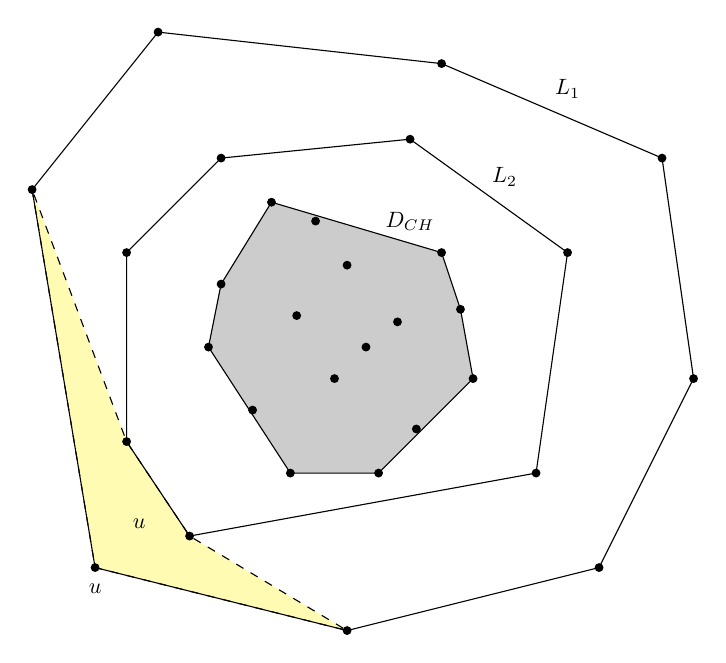
\begin{tikzpicture}[scale=0.8, every node/.style={transform shape}]
        % Define coordinates for the points
        % D_CH: Innermost points
        \coordinate (dch1) at (-0.5, 2.5);
        \coordinate (dch2) at (-2, 1.5);
        \coordinate (dch3) at (-1.5, -0.5);
        \coordinate (dch4) at (0.5, -1.5);
        \coordinate (dch5) at (2, 0);
        \coordinate (dch6) at (1.5, 2);
        \coordinate (dch7) at (-0.8, 1);
        \coordinate (dch8) at (-0.2, 0);
        \coordinate (dch9) at (0.8, 0.9);
        % --- Additional interior points ---
        \coordinate (dch10) at (0, 1.8);
        \coordinate (dch11) at (-1.2, 2.8);
        \coordinate (dch12) at (1.1, -0.8);
        \coordinate (dch13) at (-2.2, 0.5);
        \coordinate (dch14) at (0.3, 0.5);
        \coordinate (dch15) at (1.8, 1.1);
        \coordinate (dch16) at (-0.9, -1.5);

        % L2: Second convex layer
        \coordinate (l2-1) at (-2, 3.5);
        \coordinate (l2-2) at (-3.5, 2);
        \coordinate (l2-3) at (-3.5, -1);
        \coordinate (l2-4) at (-2.5, -2.5);
        \coordinate (l2-5) at (3, -1.5);
        \coordinate (l2-6) at (3.5, 2);
        \coordinate (l2-7) at (1, 3.8);

        % L1: Outermost convex layer (the convex hull)
        \coordinate (l1-1) at (-3, 5.5);
        \coordinate (l1-2) at (-5, 3);
        %\coordinate (l1-3) at (-5.5, 0);
        \coordinate (l1-4) at (-4, -3);
        \coordinate (l1-5) at (0, -4);
        \coordinate (l1-6) at (4, -3);
        \coordinate (l1-7) at (5.5, 0);
        \coordinate (l1-8) at (5, 3.5);
        \coordinate (l1-9) at (1.5, 5);

        % --- Sensitivity highlight for point u (l1-4) ---
        % The highlighted polygon is formed by u, its neighbors, and its active points.
        \filldraw[yellow!30, draw=black, dashed] (l1-2) -- (l1-4) -- (l1-5) -- (l2-4) -- (l2-3) -- cycle;
        
        % Draw and shade the convex hull of the D_CH points
        %\filldraw[gray!40, draw=black] (dch1) -- (dch2) -- (dch3) -- (dch4) -- (dch5) -- (dch6) -- cycle;
        % Draw and shade the convex hull of the D_CH points (CCW order)
        \filldraw[gray!40, draw=black] (dch13) -- (dch16) -- (dch4) -- (dch5) -- (dch15) -- (dch6) -- (dch11) -- (dch2) -- cycle;

        % Draw the L2 polygon
        \draw (l2-1) -- (l2-2) -- (l2-3) -- (l2-4) -- (l2-5) -- (l2-6) -- (l2-7) -- cycle;

        % Draw the L1 polygon
        \draw (l1-1) -- (l1-2) -- (l1-4) -- (l1-5) -- (l1-6) -- (l1-7) -- (l1-8) -- (l1-9) -- cycle;
        
        % Draw all the points as filled circles
        \foreach \i in {1,...,16} { \fill (dch\i) circle (2pt); }
        \foreach \i in {1,...,7} { \fill (l2-\i) circle (2pt); }
        \foreach \i in {1,2,4,5,6,7,8,9} { \fill (l1-\i) circle (2pt); }

        % Add labels
        \node at (l1-4) [below=4pt] {$u$};
        \node at (-3.3, -2.3) {$\sens{u}$};
        \node at (3.5, 4.6) {$L_1$};
        \node at (2.5, 3.2) {$L_2$};
        \node at (1, 2.5) {$D_{CH}$};

    \end{tikzpicture}
    \caption{
    The data structures maintained during the peeling process. 
    The algorithm maintains the two outer convex layers, $L_1$ and $L_2$, and a dynamic convex hull data structure $D_{CH}$ for the remaining points. 
    The yellow shaded area illustrates the sensitivity $\sens{u}$ of point $u$, representing the decrease in convex hull area if $u$ were removed. 
    This area is defined by $u$, its neighbors on $L_1$, and its two active points on $L_2$.
    }
    \label{fig:peeling_datastructures_sensitivity}
\end{figure}

In each round, the priority queue determines which point is peeled. 
Then $L_1$, $L_2$, and $D_{CH}$ are updated via tangent and extreme point queries to move points from $L_2$ to $L_1$, and from $D_{CH}$ to $L_2$. 
Though many points may be moved in a single iteration, each point moves monotonically from higher to lower \emph{depth}. 
The depth of a point is defined as the number of convex layers enclosing it~\cite{1057060}. 
This allows us to charge $\Oh{\log n}$ time to each new point that appears in $L_1$ or $L_2$ after each peel, which suffices to cover the cost of updating $L_1$, $L_2$, and $D_{CH}$. 
The key technical challenge is to update the sensitivities of neighbors of the peeled point in time proportional to the number of new active points they gain. This is formalized in Lemma~\ref{lem:update-sensitivities} and combined with the bound in Theorem~\ref{thm:bounding_active_points_amortized}. 
Figure~\ref{fig:compute_new_sensitivity} shows how the active points change when a neighboring point is peeled. 

\begin{lemma}\label{lem:update-sensitivities}(Manuscript~\ref{chap:peeling}) 
    Let $(u, v)$ be points on the first layer. Consider a peel of $v$ where $\delta_u$ new points become active points for $u$.
    Then the updated sensitivity $\sens{u}$ can be computed in $\OhTheta{\delta_u + \log n}$ time, excluding the time to restore the second and first layer.
\end{lemma}


%How to efficiently implement the different steps of the high-level algorithm. 
%Mention sensitivity and the priority queue. 
%Mention the dynamic point location inner structure. 
%Mention the shoelace formulae and list-in-a-tree structure to efficiently compute areas. 
%Mention the amortized analysis bounding number of 'activations'.

\subsection{Inspiration from Biology}
Our motivation to study this problem arose from biology, specifically from geometric methods used in ecology to analyze biodiversity. 
Ecologists often represent species as points in a multidimensional trait space. 
This space is defined by characteristics such as body size, diet, or habitat preference. 
Biodiversity is then quantified using the area or volume of the convex hull enclosing these points~\cite{Cornwell_biology, Layman_biology_2}. 
In this setting, outliers correspond to species whose traits differ significantly from others, thus disproportionately enlarging the convex hull and potentially skewing ecological interpretations, including measures of biodiversity or niche variety.

Motivated by these practical biological scenarios, we considered a simplified but still challenging two-dimensional version of the problem, aiming to make statistical measures more robust to outliers. 
Given the size of ecological datasets, it was particularly important to develop a near-linear-time algorithm. 
Since our method allows efficient peeling of all points, it supports data exploration and improves interpretability. 
Plotting the area of the convex hull against the number of peeled points helps reveal the underlying structure of the data.
Although peeling algorithms are well-established in computational geometry~\cite{loffler2014unions, peeling_layers1, shamos1978thesis, eppstein2025decremental}, it was initially unclear whether an efficient solution would be possible for the area-weighted peeling problem. 
Our contribution lies in precisely formulating this biologically inspired geometric problem and proving that it admits an efficient solution. 

\subsection{Future Directions}
Several directions remain open for future work on area-weighted convex hull peeling algorithms. 
First, a natural next step is to extend the algorithm to the three-dimensional setting. 
Two major challenges are adapting both dynamic convex hull data structures and the amortized analysis of Theorem~\ref{thm:bounding_active_points_amortized} to three dimensions. 

Second, in our current formulation, all points are peeled by performing successive $1$-peels. 
A more accurate and robust approach would be to perform successive $k$-peels for values of $k > 1$, as each step would then remove a group of mutually reinforcing outliers, reducing the risk of outlier masking. 
However, even in the seemingly simple case of $k = 2$, it remains difficult to improve upon the naive strategy of repeatedly applying the exact algorithm of Atanassov et al.~\cite{2009_Atanassov_exact_small_k}, which results in a total running time of $\OhTheta{n^2 \log n}$. 

Third, it would be valuable to empirically evaluate the algorithm on real-world datasets and compare its performance with widely used methods such as Isolation Forest~\cite{4781136, 10.1145/2133360.2133363}. 
Hybrid approaches could also be explored, where convex hull peeling is applied after clustering the data, using for example $k$-center clustering~\cite{Hakimi_k_center} or Local Convex Hulls~\cite{Getz_local_convex_hull_biology}, and outliers are identified within each cluster. 
The algorithm could prioritize which clusters to peel from by maintaining a global priority queue across the clusters. 
As always with outlier detection, the appropriate choice of method ultimately depends on some prior knowledge of the data and the type of outliers that one aims to detect.

%\begin{itemize}
%    \item Challenges with adapting the solution to 3D. 3D convex hull dynamic data structure
%    \item Peeling $k$ points in $\frac{n}{k}$ rounds. How to do it in $\sim n^2$ time for $2$-peeling.
%    \item Mention challenges with theoretically defining outliers. 
    %\item Experiments and compare with fx \href{https://en.wikipedia.org/wiki/Isolation_forest}{Isolation forest}, see Credit Card Fraud Detection dataset.
    %\item Challenge "This phenomenon is known as outlier masking. Duplicates and near duplicates are natural and therefore the semantics of any anomaly detection algorithm has to accommodate them.", from \href{https://proceedings.mlr.press/v48/guha16.pdf}{Robust Random Cut Forest Based Anomaly Detection On Streams}
    %\item maybe first perform clustering and then find outliers for each cluster (fx k-center or Local Convex Hull (LoCoH)). 
%\end{itemize}


\section{The Contiguous Art Gallery Problem}
\label{sec:The Contiguous Art Gallery Problem}
The classical \emph{art gallery problem}, posed by Klee in 1973~\cite{10.5555/40599}, asks for the minimum set of guards that can be placed in a polygon such that every point within the polygon is visible to at least one guard. 
Over the decades, many variants have been studied. 
Most of these are known to be computationally hard, often being at least \textsc{NP}-hard. 
In this section, we consider the \emph{contiguous art gallery problem}, a recently introduced variant in which the goal is to partition the boundary of a simple polygon~$P$ into a minimum number of contiguous polygonal chains, each of which must be visible to a guard located within~$P$. 
We refer to each such visible portion of the boundary as a \emph{visible interval}. 
Crucially, each guard may only cover a single contiguous portion of the boundary, and neither the guard locations nor the chain endpoints are required to coincide with polygon vertices. 
This variant was posed as an open problem by Shermer in 2024 as a candidate for a tractable restriction of the art gallery problem. 

\subsection{Results}
In manuscript~\ref{chap:art_gallery}, we prove that the contiguous art gallery problem is solvable in polynomial time. 
In particular, we develop a simple greedy algorithm that always finds an optimal set of guards, as stated in Theorem~\ref{thm:CAG_is_in_P_RAM}, in the real-RAM model of computation. 

\begin{theorem}(Manuscript~\ref{chap:art_gallery} Theorem~1) 
\label{thm:CAG_is_in_P_RAM}
    There exists an algorithm for the contiguous art gallery problem for a simple polygon with $n$ vertices that determines the optimal number of guards and their placement in $\Oh{n^6\log n}$ arithmetic operations. 
\end{theorem}

We provide a \Cpp implementation of the algorithm, which is available~\cite{github_impl} and demonstrates the simplicity of the approach. 
% and based on a \Cpp implementation we find that it performs well in practice. % write this sentence better
By bounding the bit complexity of the intermediate values computed by the algorithm, we show that the problem belongs to the class \textsc{P}. 
That is, it can be solved in polynomial time on a Turing machine~\cite{turing1936computable}, as stated in Theorem~\ref{thm:CAG_is_truly_in_P}.

\begin{theorem}(Manuscript~\ref{chap:art_gallery} Theorem~2) 
\label{thm:CAG_is_truly_in_P}
    The contiguous art gallery problem for a simple polygon with vertices encoded as rational coordinates is in \textsc{P}.
\end{theorem}

The fact that this contiguous variant admits an efficient algorithm is a surprising positive result, since most art gallery-type problems are known to be \textsc{NP}-hard~\cite{10.1145/800157.805047} or even $\exists \mathbb{R}$-complete~\cite{Schaefer2017, 10.1145/62212.62257, Matousek2014}. 
Our result contributes to clarifying the boundary between tractable and intractable variants of the art gallery problem. 
Biniaz et al.\cite{biniaz2025contiguousboundaryguarding} and Robson et al.\cite{robson2025analyticarccoverproblem} independently proved the same main result, each using a different approach. 
The three approaches were subsequently unified in a joint publication~\cite{biniaz_et_al:LIPIcs.SoCG.2025.20}. 

\subsection{Related Work}
The art gallery problem has a long and well-studied history in computational geometry. 
The original version, in which guards must cover the entire polygon, is \textsc{NP}-hard when guards are restricted to vertices, as shown by Lee and Lin~\cite{Lee1990}. 
The edge-covering variant, in which only the boundary must be guarded, is also \textsc{NP}-hard for vertex guards, as shown by Laurentini~\cite{Laurentini1999}. 
The unrestricted versions of both the original and edge-covering problems, where guards may be placed anywhere in simple polygons (possibly with holes), are $\exists\mathbb{R}$-complete~\cite{10.1145/3486220}. 
In the tractable direction, Abrahamsen et al.~\cite{10.1145/3618260.3649756} showed that the minimum star-shaped partition problem can be solved using $\Oh{n^{105}}$ arithmetic operations. 
When the star-shaped regions are restricted to use only vertices of the input polygon, the complexity improves to $\Oh{n^7 \log n}$ operations~\cite{doi:10.1137/0214056}. 
The minimum star-shaped partition problem is \textsc{NP}-hard for polygons with holes~\cite{10.5555/40599}. 
A common theme across variants is that restricting guard positions and coverage regions to discrete locations, such as vertices of the input polygon, often reduces the complexity to membership in \textsc{P}. 
In contrast, for polygons with holes, many variants are at least \textsc{NP}-hard. 

The contiguous variant is closely related to the \emph{circular arc covering} problem, which asks for a minimum-size subset among $m$ arcs that covers a circle, and can be solved in $\Oh{m \log m}$ time~\cite{LEE1984109}. 
In our setting, the polygon boundary can be interpreted as a distorted circle, and an optimal guard cover corresponds to covering the boundary with visible intervals, each mapped to an arc on the circle. 
If the set of candidate visible intervals were finite and explicitly known, the Lee and Lee arc-covering algorithm could be applied directly. 
The difficulty lies in the fact that the number of candidate visible intervals may be infinite, as illustrated in Figure~\ref{fig:CAG_tradeoff_infinite_different}. 
Surprisingly, we show that the same greedy strategy used by Lee and Lee also yields an optimal solution in our setting. 
The strategy repeatedly selects the arc, or in our case the visible interval, that extends furthest along the boundary from the current position. 
In their setting, the arcs are given explicitly. 
In our geometric setting, each visible interval implicitly defines an arc. 

\begin{figure}[ht]
    \centering

    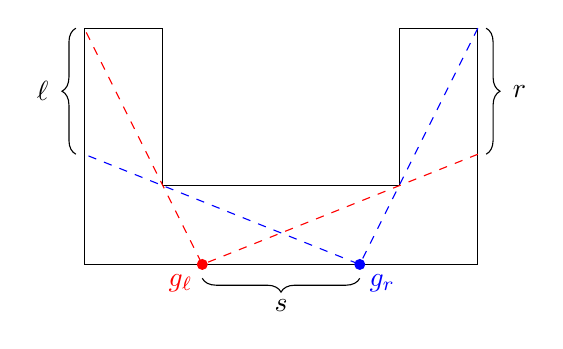
\begin{tikzpicture}
        \draw (0, 0) -- (-5, 0) -- (-5, 3) -- (-4, 3) -- (-4, 1) -- (-1, 1) -- (-1, 3) -- (0, 3) -- cycle;
        \fill[color=blue] (-1.5, 0) circle[radius=0.07] node[below right] {\textcolor{blue}{$g_r$}};
        \fill[color=red] (-3.5, 0) circle[radius=0.07]  node[below left] {\textcolor{red}{$g_\ell$}};;
        \draw[dashed, color=blue] (0, 3) -- (-1.5, 0) -- (-5, 1.4);
        \draw[dashed, color=red] (0, 1.4) -- (-3.5, 0) -- (-5, 3);
        \draw [decorate,decoration={brace,amplitude=5pt,raise=3pt}]
                (0, 3) -- node[xshift=15pt] {$r$} (0, 1.4);
        \draw [decorate,decoration={brace,amplitude=5pt,raise=3pt}]
                (-5, 1.4) -- node[xshift=-15pt] {$\ell$} (-5, 3);
        \draw [decorate,decoration={brace,amplitude=5pt,raise=5pt}]
                (-1.5, 0) -- node[yshift=-15pt] {$s$} (-3.5, 0);
    \end{tikzpicture}
    
    \caption{
    (Manuscript~\ref{chap:art_gallery} Figure~2) A polygon where the blue guard $g_r$ sees all of $r$ and none of $\ell$, and the red guard $g_\ell$ sees all of $\ell$ and none of $r$. 
    Any guard placed along the segment $s$ yields a trade-off between how much of $\ell$ and $r$ it can see. 
    This illustrates that, with unrestricted guard placements, it is non-trivial to extract a finite candidate set of visible intervals.
    }
    \label{fig:CAG_tradeoff_infinite_different}
\end{figure}

\subsection{The Simple Greedy Algorithm}
%1) Based on primitive opeartion "GreedyInterval" which ...
%2) pseudo-code, repeat k = ... times
%3) analysis based no local greedy sequences and stopping conditions such as ...
% brief mention of others
\todo{example run figure?}
At the heart of our solution is the primitive operation \textsc{GreedyInterval}$(x)$. 
Given a starting point $x$ on the boundary of $P$, this operation computes the longest contiguous boundary interval $[x,y]$ in the clockwise direction that is visible from a guard point $g$ located in the interior of the polygon. 
That is, \textsc{GreedyInterval} extends forward from $x$ along the boundary of the polygon until visibility is obstructed by the geometry. 
The operation returns the endpoint $y$ of the visible interval, along with a guard position $g$ that sees the entire interval $[x,y]$. 
A greedy interval can be computed in polynomial time using standard computational geometry procedures such as constructing visibility polygons~\cite{1675729, ELGINDY1981186}, computing polygon intersections~\cite{10.1145/563858.563896}, and finding common tangents~\cite{10.1145/3284355}. 

\begin{algorithm}[ht]
    \caption{\label{alg:greedy} (Manuscript~\ref{chap:art_gallery} Algorithm~1)}
    \KwIn{A simple polygon $P$ with vertices $v_0, v_1, v_2, \dots, v_n$}
    \KwOut{An explicit solution to the contiguous art gallery problem for $P$}
    $x_0 \longleftarrow v_0$\\
    \nllabel{line:start} \For{$i=1$ \KwTo $T$} {
        \nllabel{line:loop_greedy_interval1} $x_i, g_i \longleftarrow GreedyInterval\!\parentheses{x_{i - 1}, P}$ \\
    }
    \nllabel{line:loop_greedy_interval2} $j \longleftarrow \myMax{j \leq T - 2}{x_j \in \left( x_{T - 1}, x_T \right] }$ \\
    \nllabel{line:return_last_segments1} 
    \Return $\curlyBrackets{\parentheses{x_{i - 1}, x_i, g_i} |\; j < i \leq T}$ \tcp*[ht]{The last segments/guards covering the boundary of $P$} 
    \nllabel{line:return_last_segments2}
\end{algorithm}

Algorithm~\ref{alg:greedy} iterates the subroutine \textsc{GreedyInterval} $T$ times, where $T$ is a parameter, thereby traversing the boundary of the polygon.
A single traversal proceeds as follows. 
The algorithm begins at a boundary point $x_0$ and performs $\textsc{GreedyInterval}(x_0)$ to compute a maximal initial segment. 
The endpoint of this segment is denoted $x_1$. 
It then performs $\textsc{GreedyInterval}(x_1)$ to cover the next segment, and continues in this manner. 
The traversal eventually reaches a point beyond $x_0$, indicating that the entire boundary is covered by the sequence of visible segments $[x_0,x_1], [x_1,x_2], \ldots, [x_{k-1},x_k]$.	 
If the first pass uses $k$ guards, we prove that this number is at most one more than the optimal, following a similar argument to that of Lee and Lee~\cite{LEE1984109}.	 

Our main technical result is the proof that $T = \OhTheta{n^4}$ revolutions suffice for Algorithm~\ref{alg:greedy} to return an optimal solution. 
This bound on the number of iterations is the essential component in establishing the total runtime complexity stated in Theorem~\ref{thm:CAG_is_in_P_RAM}. 
The need for multiple revolutions arises because after the initial, possibly suboptimal pass, the algorithm may reduce the number of guards by one to reach optimality. 
To show this, we first characterize the combinatorial behavior of the endpoints generated by repeated applications of the \textsc{GreedyInterval} algorithm. 
We prove that if the sequence is \emph{optimal}, then it remains optimal in further iterations. 
A sequence is optimal if it contains a consecutive set of guard intervals of optimal size that cover the boundary of $P$. 
Second, if the sequence is not optimal, then its endpoints can be restricted to certain fixed intervals of the boundary. 
Within each such interval, the endpoints move monotonically in the counterclockwise direction, as illustrated in Figure~\ref{fig:local_seq_art_gall}. 
We translate this behavior into a set of geometric conditions on the sequence of endpoints, which can be used to certify optimality. 
These conditions include a violation of monotonicity within an interval, repetition of an endpoint, or the sequence passing more than $n + 1$ vertices along the boundary of $P$. 

\begin{figure}[ht]
    \centering
    
    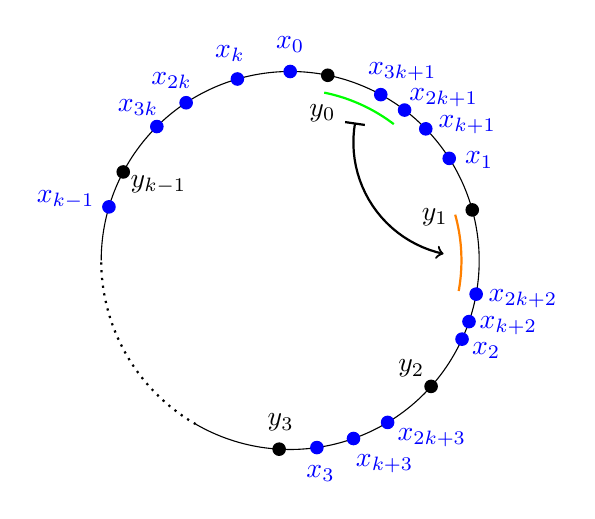
\begin{tikzpicture}[scale=0.75]
        \draw (-120:3.2) arc (-120:180:3.2);
        \draw[dotted, thick] (-120:3.2) arc (-120:-180:3.2);
        \filldraw[color=blue] (0.000, 3.200) circle (3pt); % angle = 90.000
        \draw[blue] (0.000, 3.650) node {$x_0$};
        \filldraw[color=blue] (2.693, 1.729) circle (3pt); % angle = 32.704
        \draw[blue] (3.200, 1.700) node {$x_1$};
        \filldraw[color=blue] (2.910, -1.332) circle (3pt); % angle = -24.592
        \draw[blue] (3.319, -1.519) node {$x_2$};
        \filldraw[color=blue] (0.452, -3.168) circle (3pt); % angle = -81.887
        \draw[blue] (0.515, -3.613) node {$x_3$};
        \filldraw[color=blue] (-3.069, 0.908) circle (3pt); % angle = -196.479
        \draw[blue] (-3.800, 1.035) node {$x_{k-1}$};
        \filldraw[color=blue] (-0.894, 3.073) circle (3pt); % angle = -253.775
        \draw[blue] (-1.020, 3.505) node {$x_{k}$};
        \filldraw[color=blue] (2.296, 2.229) circle (3pt); % angle = 44.163
        \draw[blue] (3.000, 2.300) node {$x_{k+1}$};
        \filldraw[color=blue] (1.937, 2.547) circle (3pt); % angle = 52.758
        \draw[blue] (2.600, 2.750) node {$x_{2k+1}$};
        \filldraw[color=blue] (1.534, 2.808) circle (3pt); % angle = 61.352
        \draw[blue] (1.900, 3.200) node {$x_{3k+1}$};
        \filldraw[color=blue] (3.028, -1.035) circle (3pt); % angle = -18.862
        \draw[blue] (3.694, -1.100) node {$x_{k+2}$};
        \filldraw[color=blue] (3.149, -0.570) circle (3pt); % angle = -10.268
        \draw[blue] (3.942, -0.651) node {$x_{2k+2}$};
        \filldraw[color=blue] (1.072, -3.015) circle (3pt); % angle = -70.428
        \draw[blue] (1.600, -3.439) node {$x_{k+3}$};
        \filldraw[color=blue] (1.650, -2.742) circle (3pt); % angle = -58.969
        \draw[blue] (2.400, -3.000) node {$x_{2k+3}$};
        \filldraw[color=blue] (-1.762, 2.671) circle (3pt); % angle = -236.586
        \draw[blue] (-2.010, 3.047) node {$x_{2k}$};
        \filldraw[color=blue] (-2.258, 2.268) circle (3pt); % angle = -225.127
        \draw[blue] (-2.575, 2.587) node {$x_{3k}$};
        \filldraw[color=black] (0.636, 3.136) circle (3pt); % angle = 78.541
        \draw[black] (0.546, 2.495) node {$y_0$};
        \filldraw[color=black] (3.083, 0.856) circle (3pt); % angle = 15.515
        \draw[black] (2.450, 0.736) node {$y_1$};
        \filldraw[color=black] (2.386, -2.132) circle (3pt); % angle = -41.780
        \draw[black] (2.051, -1.832) node {$y_2$};
        \filldraw[color=black] (-0.187, -3.195) circle (3pt); % angle = -93.346
        \draw[black] (-0.161, -2.745) node {$y_3$};
        \filldraw[color=black] (-2.827, 1.499) circle (3pt); % angle = -207.938
        \draw[black] (-2.230, 1.288) node {$y_{k-1}$};

        \draw[green, thick, domain = 78.541: 52.758] plot ({2.9*cos(\x)}, {2.9*sin(\x)});
        \draw[orange, thick, domain = 15.515: -10.268] plot ({2.9*cos(\x)}, {2.9*sin(\x)});

        \draw[black, thick, domain = -190.08:-102.06, |->] plot ({1.93*cos(\x)+3}, {1.93*sin(\x)+2}); 
        %\draw[black] (-0.5,0.6) node {\small \textsc{GreedyInterval}};
    \end{tikzpicture}
    
    \caption{(Manuscript~\ref{chap:art_gallery} Figure~18) The boundary of $P$ visualized as a circle, where the $y_i$'s indicate the endpoints of an optimal solution. 
    The $x_i$'s indicate a non-optimal sequence of endpoints generated by repeatedly running \textsc{GreedyInterval}, starting from $x_0$ and the last point generated being $x_{3k +1}$. 
    If the sequence remains non-optimal, it maps points from $[y_0,x_{2k+1}]$ (green) to $[y_1,x_{2k+2}]$ (orange), and in the next revolution from  $[y_0,x_{3k+1}]$ to $[y_1,x_{3k + 2}]$.}
    \label{fig:local_seq_art_gall}
\end{figure}

\subsection{Discussion}
% conjecture constant number of revolutions enough (experiments suggest)

Empirical evidence suggests that the greedy algorithm is not only polynomial in theory but also highly efficient in practice. 
In extensive experiments on random polygons, the algorithm never required the worst-case bound of $\Oh{n^4}$ revolutions around the boundary. 
In fact, in more than two million random tests, an optimal solution was always obtained within \emph{four} revolutions. 
Thus, we pose the conjecture that a constant number of revolutions suffices to find an optimal solution. 
Extending the algorithm to polygons with holes, or proving that this generalization is computationally hard, remains a natural open problem. 




